% ============================================================
% Section 3 — Method
% ============================================================
\section{HAT: Hippocampus-Augmented Transformer}
\label{sec:method}

We present \textbf{Hippocampus-Augmented Transformer (HAT)}, a memory-centric continual learning approach that enables language models to learn \emph{what to learn} from interaction.
HAT is inspired by hippocampal--neocortical memory consolidation in the mammalian brain, where salient experiences are rapidly encoded, selectively retained, and later replayed for gradual integration into long-term cortical memory.
Rather than updating a model from all observed interactions, HAT separates online experience acquisition from offline model adaptation: during the \emph{wake phase}, interaction traces are selectively consolidated into a long-term memory; during the \emph{slow-wave sleep} (SWS) phase, selected traces are replayed as training signals to update the model.

As shown in Figure~\ref{fig:architecture}, HAT consists of four functional components.
The \textbf{Cortex} $\modeltheta$ is a lightweight language model that interacts with users.
The \textbf{Hippocampus Agent} $\hippocampus$ abstracts interactions into structured memory traces, estimates their learning value, and determines whether they should be retained.
The \textbf{Neocortex} $\neocortex$ is a persistent long-term memory that stores selected traces and their replay-ready training forms.
The \textbf{SWS Trainer} periodically updates the Cortex by replaying curated memories from the Neocortex.
An external \textbf{Oracle} $\oracle$ may be queried on demand when the Cortex is uncertain or when user feedback indicates an error.

\begin{figure}[t]
  \centering
  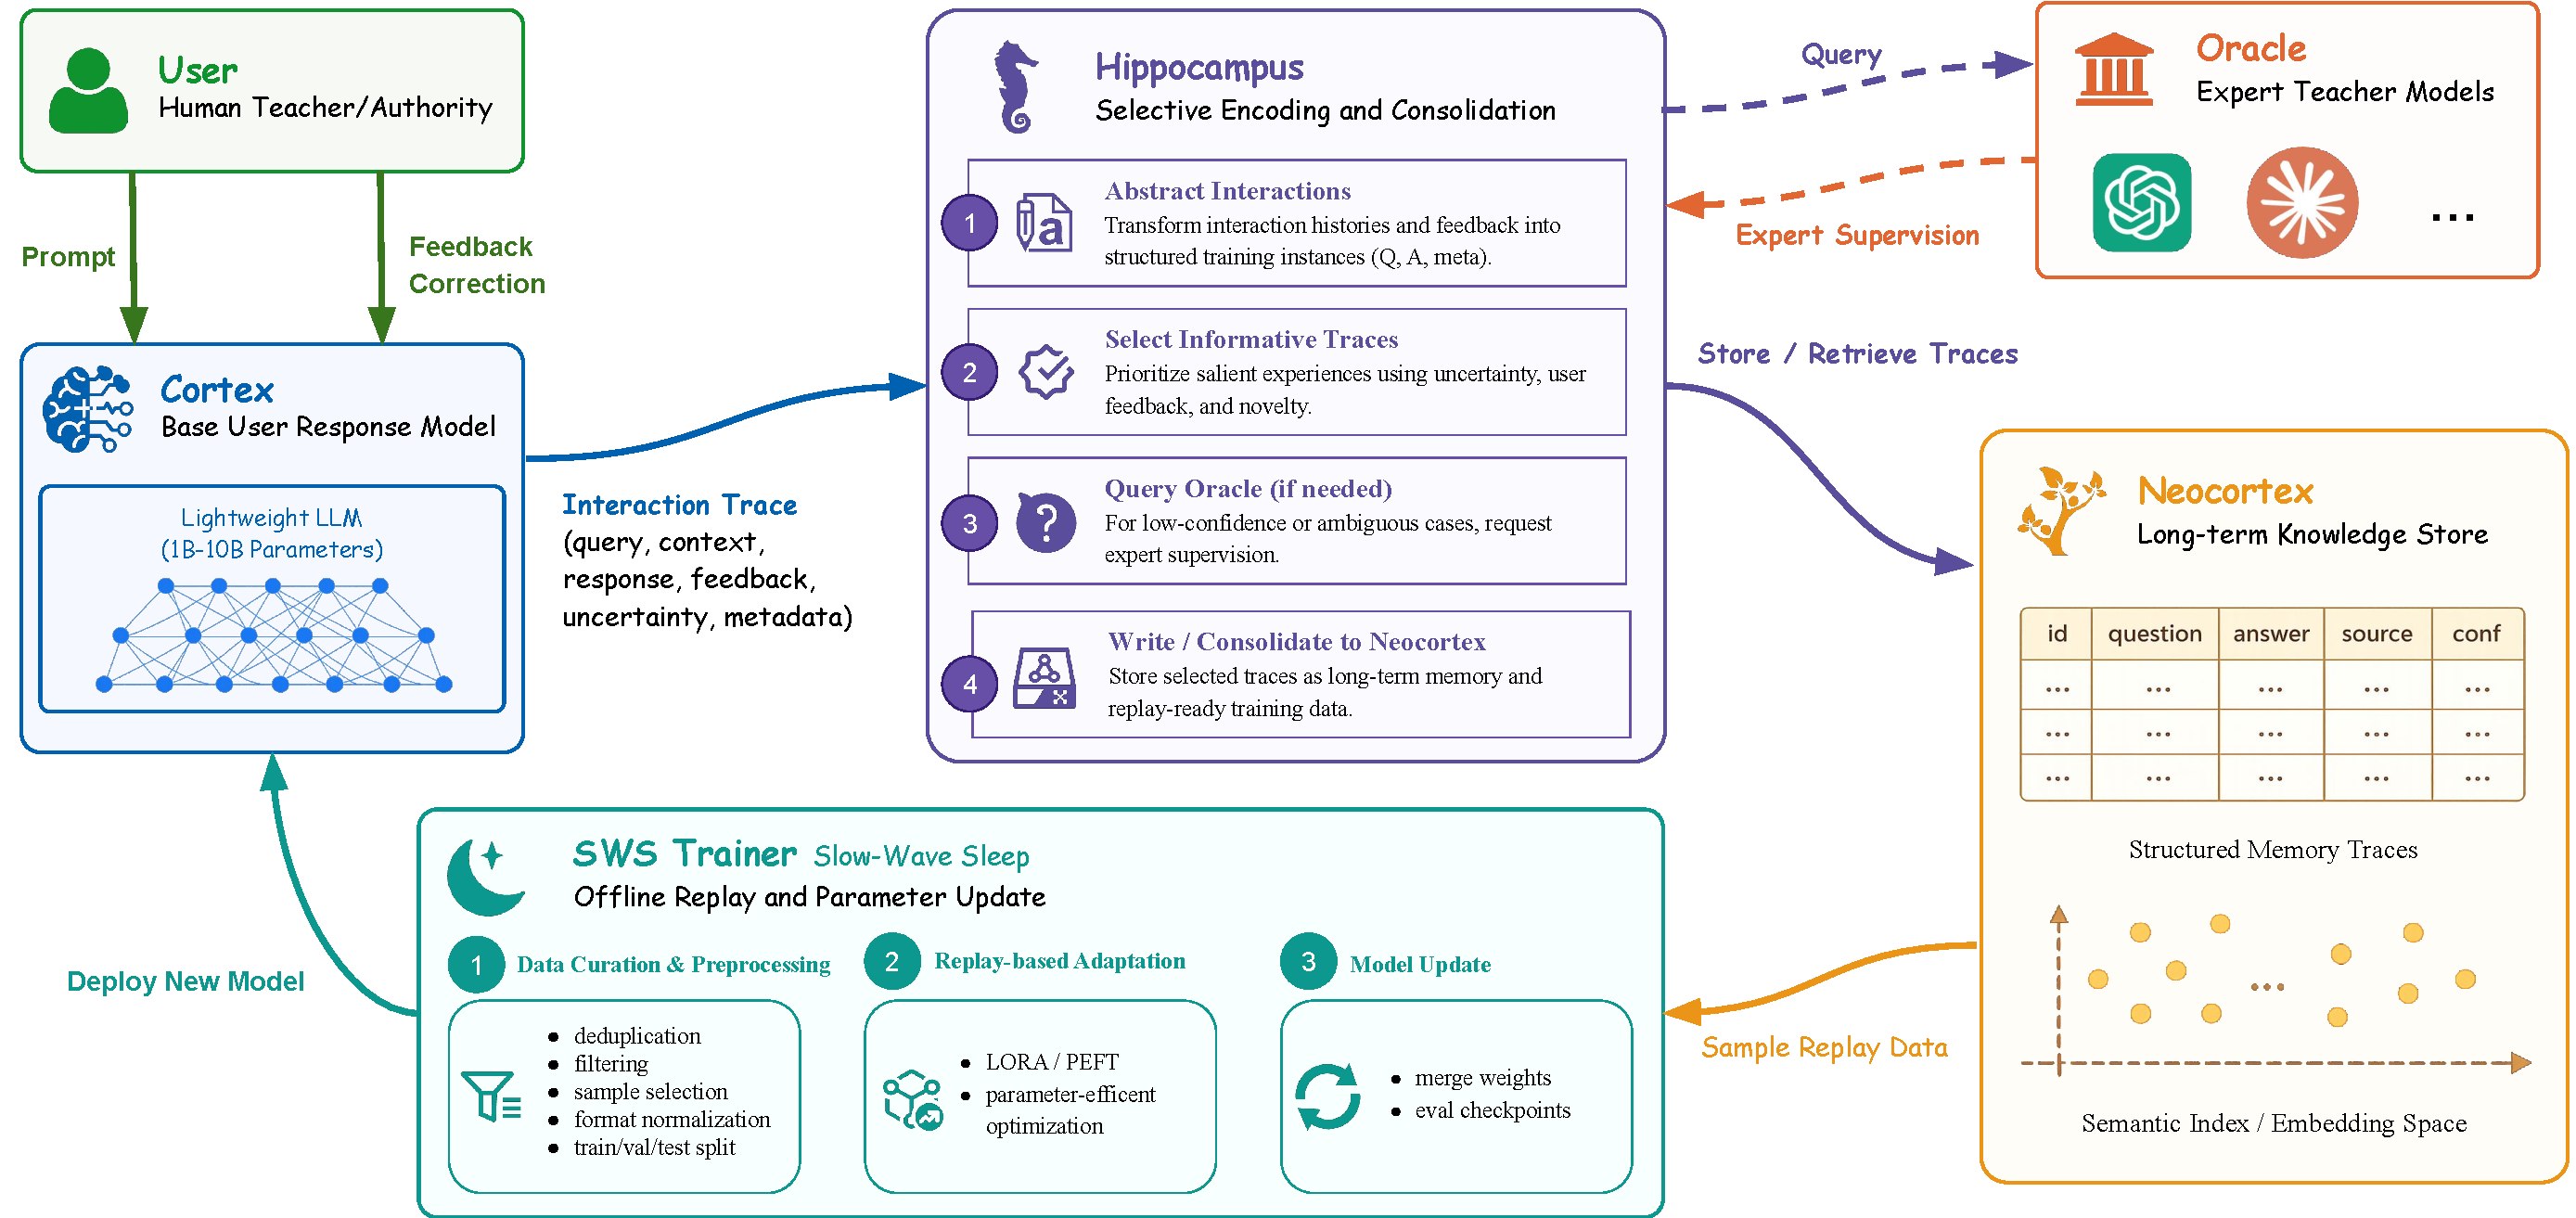
\includegraphics[width=\linewidth]{figures/framework.pdf}
  \caption{
    Overview of HAT, a hippocampus-inspired continual learning mechanism that converts selected interaction experiences into reusable training signals.
    During wake-phase interaction, the Cortex responds to user prompts while the Hippocampus encodes, selects, and optionally augments informative traces with Oracle supervision.
    The selected traces are consolidated into the Neocortex and replayed during slow-wave sleep (SWS), where the SWS Trainer updates the Cortex through parameter-efficient fine-tuning for continual self-improvement.
  }
  \label{fig:architecture}
\end{figure}

% ────────────────────────────────────────────────────────────
\subsection{Selective Learning Formulation}
\label{sec:method:formulation}

HAT treats continual adaptation as a selective learning problem over an interaction stream.
Let
\begin{equation}
  \mathcal{D}^{(t)} = \{x_i\}_{i=1}^{T_t}
\end{equation}
denote the set of interactions observed during wake cycle $t$, where each interaction is represented as
\begin{equation}
  x_i = (\context_i, \seq_i, \seqy_i, f_i),
\end{equation}
with context $\context_i$, user query $\seq_i$, model response $\seqy_i$, and optional feedback signal $f_i$.
The goal is not to learn from every interaction, but to identify a subset of experiences that are likely to improve the model under a limited adaptation budget.

Ideally, one would select experiences according to their expected learning gain:
\begin{equation}
  \mathcal{D}^{*(t)}
  =
  \arg\max_{\mathcal{D}' \subseteq \mathcal{D}^{(t)}}
  \;
  \mathbb{E}_{x \sim \mathcal{D}'}
  \left[
    \Delta \mathcal{L}(\params; x)
    \right],
  \label{eq:ideal_selection}
\end{equation}
where $\Delta \mathcal{L}(\params; x)$ denotes the expected reduction in future loss after adapting the model on experience $x$.
Since this quantity is generally unobservable at selection time, HAT approximates expected learning gain using observable proxies:
model uncertainty, external feedback, and semantic novelty.
This converts continual learning from indiscriminate data accumulation into a selective memory consolidation process.

% ────────────────────────────────────────────────────────────
\subsection{Wake--Sleep Learning Cycle}
\label{sec:method:wake_sleep}

HAT alternates between two complementary phases.

\paragraph{Wake phase.}
During the wake phase, the Cortex $\modeltheta$ receives a user query $\seq$ under context $\context$ and generates a response $\seqy$.
The resulting interaction is passed to the Hippocampus Agent, which compresses it into a memory trace, evaluates its utility, and determines whether it should be consolidated into the Neocortex.
If the Cortex is uncertain or the user provides corrective feedback, the Hippocampus Agent may consult the Oracle to obtain additional supervision.

\paragraph{Sleep phase.}
During the SWS phase, selected traces stored in the Neocortex are replayed as training examples.
The SWS Trainer updates the Cortex parameters using a curated replay distribution:
\begin{equation}
  \params^{(t+1)}
  =
  \mathrm{SWS}
  \left(
  \params^{(t)}, \neocortex^{(t)}
  \right).
  \label{eq:sws_transition}
\end{equation}
The updated model then becomes the Cortex for the next wake cycle.
Thus, HAT separates the decision of \emph{what should be learned} from the optimization process that performs the actual learning.

% ────────────────────────────────────────────────────────────
\subsection{Cortex: Online Interaction Model}
\label{sec:method:cortex}

The Cortex is an autoregressive Transformer language model $\modeltheta$ with parameters $\params$.
It can be instantiated by any lightweight model suitable for deployment, such as a model in the 0.5--10B parameter range.
Given context $\context$ and query $\seq$, the Cortex generates a response $\seqy = (y_1,\ldots,y_{|\seqy|})$ according to
\begin{equation}
  p_{\params}(\seqy \mid \context, \seq)
  =
  \prod_{j=1}^{|\seqy|}
  p_{\params}
  \left(
  y_j \mid \context, \seq, \seqy_{<j}
  \right).
  \label{eq:autoregressive}
\end{equation}

In addition to producing a response, the Cortex provides an uncertainty estimate $U(x)$ for each interaction.
In practice, $U(x)$ can be computed from predictive entropy, token-level confidence, self-consistency variance, or disagreement between sampled generations.
A simple entropy-based estimate is
\begin{equation}
  U(x)
  =
  \frac{1}{|\seqy|}
  \sum_{j=1}^{|\seqy|}
  H
  \left(
  p_{\params}
  (\cdot \mid \context, \seq, \seqy_{<j})
  \right),
  \label{eq:uncertainty}
\end{equation}
where $H(\cdot)$ denotes entropy.
High uncertainty indicates a potential epistemic gap and serves as one signal for selective memory consolidation.

% ────────────────────────────────────────────────────────────
\subsection{Hippocampus Agent: Selective Memory Consolidation}
\label{sec:method:hippocampus}

The Hippocampus Agent is the central mechanism of HAT.
It transforms raw interactions into structured memory traces and determines which traces should be consolidated into the Neocortex.
This process consists of three operations: abstraction, selection, and replay construction.

% --- 3.x.1 Abstraction ---
\subsubsection{Experience Abstraction}
\label{sec:method:abstraction}

Raw interaction logs are often verbose, redundant, and unsuitable for direct training.
The abstraction operation maps an interaction $x = (\context,\seq,\seqy,f)$ into a compact memory trace:
\begin{equation}
  \memtrace
  =
  \hippocampus_{\mathrm{abs}}
  (\context,\seq,\seqy,f).
  \label{eq:abstraction}
\end{equation}
The trace $\memtrace$ preserves the learning-relevant content of the episode, including the user intent, the model response, the corrected answer if available, and relevant contextual constraints.
This operation is analogous to rapid hippocampal encoding, where an experience is compressed into a retrievable trace rather than stored as an unfiltered sensory stream.

In implementation, $\hippocampus_{\mathrm{abs}}$ can be instantiated as a prompting procedure, a small summarization model, or the Cortex itself under an instruction template.
A memory trace may be represented as
\begin{equation}
  \memtrace
  =
  \left(
  q,\;
  a_{\mathrm{cortex}},\;
  a_{\mathrm{target}},\;
  r,\;
  \metadata
  \right),
  \label{eq:memory_trace}
\end{equation}
where $q$ is the normalized query, $a_{\mathrm{cortex}}$ is the Cortex response, $a_{\mathrm{target}}$ is the preferred target answer, $r$ is the rationale or correction signal, and $\metadata$ contains timestamp, source, uncertainty, feedback, and novelty statistics.

% --- 3.x.2 Selection ---
\subsubsection{Selection via Write Policy}
\label{sec:method:selection}

Not all traces should be stored or replayed.
HAT therefore defines a write policy $\writepolicy$ that estimates the consolidation value of each memory trace.
Given a trace $\memtrace$, the policy computes
\begin{equation}
  \mathrm{score}(\memtrace)
  =
  \alpha U(\memtrace)
  +
  \beta F(\memtrace)
  +
  \gamma N(\memtrace),
  \label{eq:selection_score}
\end{equation}
where $U$, $F$, and $N$ denote uncertainty, feedback, and novelty, respectively.

\paragraph{Uncertainty.}
$U(\memtrace)$ estimates the extent to which the Cortex is unreliable on the corresponding interaction.
High uncertainty suggests that the trace lies near the boundary of the model's current competence and may yield high learning value.

\paragraph{Feedback.}
$F(\memtrace)$ captures explicit or implicit supervision.
For example, user corrections, negative ratings, or contradiction signals can be mapped to a binary or graded value.
When an explicit correction is provided, $F(\memtrace)$ is assigned high priority to ensure that verified errors are consolidated.

\paragraph{Novelty.}
$N(\memtrace)$ measures the semantic distance between the current trace and the existing Neocortex memory.
Let $e(\memtrace)$ be an embedding of the trace and $\neocortex$ be the current memory store.
A practical novelty score is
\begin{equation}
  N(\memtrace)
  =
  1 -
  \max_{\memtrace' \in \neocortex}
  \cos
  \left(
  e(\memtrace), e(\memtrace')
  \right).
  \label{eq:novelty}
\end{equation}
Novel traces are prioritized because they expand coverage of underrepresented regions in the model's knowledge space.

The final write decision is
\begin{equation}
  z(\memtrace)
  =
  \mathbbm{1}
  \left[
    \mathrm{score}(\memtrace) > \tau
    \right],
  \label{eq:write_decision}
\end{equation}
where $\tau$ is a tunable consolidation threshold.
The coefficients $\alpha,\beta,\gamma$ control the relative importance of epistemic uncertainty, external supervision, and semantic coverage.

This write policy can be interpreted as a tractable surrogate for Equation~\ref{eq:ideal_selection}: uncertainty approximates knowledge gaps, feedback identifies externally verified errors, and novelty encourages memory diversity.

% --- 3.x.3 Replay Construction ---
\subsubsection{Replay Construction}
\label{sec:method:replay}

Selected memory traces must be converted into training-ready signals.
For each retained trace $\memtrace$, the Replay Builder produces one or more supervised examples:
\begin{equation}
  (\seq^{\mathrm{train}}, \seqy^{\mathrm{train}})
  \sim
  p_{\mathrm{replay}}(\cdot \mid \memtrace)
  =
  \hippocampus_{\mathrm{replay}}(\memtrace).
  \label{eq:replay_distribution}
\end{equation}
The replay distribution can include direct instruction--response pairs, corrected QA pairs, rationale-augmented examples, or contrastive pairs that distinguish the original erroneous response from the preferred target.

This step is important because memory consolidation in HAT is not merely storage.
A retained trace becomes useful only when it is transformed into a form that can drive gradient-based learning.
Thus, the Hippocampus Agent converts interaction experience into reusable training signals.

% ────────────────────────────────────────────────────────────
\subsection{Oracle: On-Demand External Supervision}
\label{sec:method:oracle}

The Oracle $\oracle$ is an external teacher used only when additional supervision is expected to be valuable.
Rather than distilling a large teacher model over an entire corpus, HAT queries the Oracle selectively.
The Oracle is invoked when the uncertainty exceeds a threshold $\tau_{\oracle}$ or when user feedback indicates an error:
\begin{equation}
  \seqy^{\oracle}
  =
  \oracle(\context,\seq),
  \quad
  \text{if }
  U(x) > \tau_{\oracle}
  \text{ or }
  F(x) > 0.
  \label{eq:oracle_query}
\end{equation}

The Oracle response may replace, refine, or supplement the Cortex response in the memory trace:
\begin{equation}
  a_{\mathrm{target}}
  =
  \mathrm{Merge}
  \left(
  a_{\mathrm{cortex}},
  a_{\mathrm{user}},
  a_{\oracle}
  \right),
  \label{eq:oracle_merge}
\end{equation}
where $a_{\mathrm{user}}$ denotes a user-provided correction when available.
This mechanism implements budget-aware supervision: teacher knowledge is acquired primarily at the frontier of the student's uncertainty or error, where it is most likely to improve future behavior.

% ────────────────────────────────────────────────────────────
\subsection{Neocortex: Long-Term Memory Store}
\label{sec:method:neocortex}

The Neocortex $\neocortex$ is a persistent memory store containing selected traces and their replay-ready training forms.
At wake cycle $t$, the memory is updated as
\begin{equation}
  \neocortex^{(t)}
  =
  \neocortex^{(t-1)}
  \cup
  \left\{
  \memtrace_i
  \;:\;
  z(\memtrace_i)=1
  \right\}.
  \label{eq:neocortex_update}
\end{equation}

Each memory entry stores both semantic content and training metadata:
\begin{equation}
  \neocortex
  =
  \left\{
  \left(
  \memtrace_i,\;
  \mathcal{R}_i,\;
  \mathrm{score}_i,\;
  \metadata_i
  \right)
  \right\}_{i=1}^{|\neocortex|},
  \label{eq:neocortex_structure}
\end{equation}
where $\mathcal{R}_i$ denotes replay examples generated from trace $\memtrace_i$.
In implementation, the Neocortex can be realized as a vector-indexed datastore with structured fields, allowing retrieval, deduplication, pruning, and replay sampling.

To keep memory bounded, HAT may prune low-value or redundant traces:
\begin{equation}
  \neocortex
  \leftarrow
  \mathrm{TopK}
  \left(
  \neocortex,\;
  \mathrm{score}(\memtrace)
  \right),
  \label{eq:memory_prune}
\end{equation}
or apply diversity-aware sampling to avoid overrepresenting frequent interaction patterns.
This prevents indiscriminate accumulation and maintains the Neocortex as a curated long-term learning substrate.

% ────────────────────────────────────────────────────────────
\subsection{Slow-Wave Sleep Trainer}
\label{sec:method:sws}

During the SWS phase, HAT updates the Cortex by replaying selected experiences from the Neocortex.
Let $\replaybuf \subseteq \neocortex$ denote a replay batch sampled from the memory store.
The SWS Trainer performs empirical risk minimization over the curated replay distribution:
\begin{equation}
  \min_{\params}
  \;
  \mathbb{E}_{(\seq,\seqy) \sim p_{\mathrm{replay}}}
  \left[
  \mathcal{L}_{\mathrm{sup}}
  (\params;\seq,\seqy)
  \right]
  +
  \mathcal{R}(\params).
  \label{eq:sws_erm}
\end{equation}

In practice, the supervised loss is the token-level negative log-likelihood:
\begin{equation}
  \mathcal{L}_{\mathrm{sup}}
  =
  -
  \frac{1}{|\replaybuf|}
  \sum_{(\seq,\seqy)\in \replaybuf}
  \sum_{j=1}^{|\seqy|}
  \log
  p_{\params}
  \left(
  y_j
  \mid
  \seq,\seqy_{<j}
  \right).
  \label{eq:ce_loss}
\end{equation}

For traces involving Oracle supervision, HAT optionally includes a distillation term:
\begin{equation}
  \mathcal{L}_{\mathrm{KD}}
  =
  \frac{1}{|\replaybuf_{\oracle}|}
  \sum_{\seq \in \replaybuf_{\oracle}}
  \mathrm{KL}
  \left(
  p_{\oracle}(\cdot \mid \seq)
  \,\Vert\,
  p_{\params}(\cdot \mid \seq)
  \right),
  \label{eq:kd_loss}
\end{equation}
where $\replaybuf_{\oracle}$ is the subset of replay examples that contain Oracle-derived targets.

To reduce catastrophic forgetting, the SWS objective may include a stability regularizer:
\begin{equation}
  \mathcal{L}_{\mathrm{stab}}
  =
  \frac{\mu}{2}
  \sum_i
  F_i
  \left(
  \theta_i - \theta_i^{\mathrm{old}}
  \right)^2,
  \label{eq:stability_loss}
\end{equation}
where $F_i$ denotes the estimated importance of parameter $\theta_i$, such as the diagonal Fisher information as in elastic weight consolidation~\citep{kirkpatrick2017overcoming}.

The full SWS objective is
\begin{equation}
  \mathcal{L}_{\mathrm{SWS}}
  =
  \mathcal{L}_{\mathrm{sup}}
  +
  \lambda_{\mathrm{KD}}
  \mathcal{L}_{\mathrm{KD}}
  +
  \lambda_{\mathrm{stab}}
  \mathcal{L}_{\mathrm{stab}}.
  \label{eq:sws_loss}
\end{equation}

The Cortex parameters are then updated as
\begin{equation}
  \params^{(t+1)}
  =
  \params^{(t)}
  -
  \eta
  \nabla_{\params}
  \mathcal{L}_{\mathrm{SWS}}
  \left(
  \params^{(t)};
  \replaybuf^{(t)}
  \right).
  \label{eq:sws_update}
\end{equation}
For efficient deployment, HAT can instantiate this update using parameter-efficient fine-tuning methods such as LoRA or adapters, while keeping most model parameters frozen.
This makes the SWS phase practical for small or edge-deployed language models.

% ────────────────────────────────────────────────────────────
\subsection{Iterative Self-Improvement}
\label{sec:method:loop}

The complete HAT process forms a recurrent wake--sleep learning loop.
At cycle $t$, the current Cortex interacts with users and produces an interaction stream $\mathcal{D}^{(t)}$.
The Hippocampus Agent abstracts and filters this stream into selected memory traces.
The Neocortex stores these traces as long-term memory.
The SWS Trainer then replays the selected traces to produce the next Cortex:
\begin{equation}
  \params^{(t+1)}
  =
  \mathcal{A}
  \left(
  \params^{(t)},
  \writepolicy
  \left(
    \mathcal{D}^{(t)}, \neocortex^{(t)}
    \right)
  \right),
  \label{eq:iterative_update}
\end{equation}
where $\mathcal{A}$ denotes the SWS adaptation operator and $\writepolicy$ denotes the selective consolidation policy.

This loop creates a self-improving process in which each model generation produces new interaction evidence, the Hippocampus Agent decides which experiences are worth retaining, and the SWS phase converts retained experiences into parameter updates.
Importantly, HAT does not require the model to store all interactions or continuously update online.
Instead, it learns through selective consolidation: wake-phase interactions determine \emph{what} should be learned, while sleep-phase replay determines \emph{how} the model is updated.

Algorithm~\ref{alg:hat} summarizes the full procedure.

\begin{algorithm}[t]
  \caption{HAT wake--sleep learning loop}
  \label{alg:hat}
  \DontPrintSemicolon
  \KwIn{Initial Cortex parameters $\params^{(0)}$, Neocortex memory $\neocortex^{(0)}$, Oracle $\oracle$, thresholds $\tau,\tau_{\oracle}$}
  \For{wake--sleep cycle $t = 0,1,2,\ldots$}{
  Collect wake-phase interactions $\mathcal{D}^{(t)}$\;
  \For{each interaction $x=(\context,\seq,\seqy,f) \in \mathcal{D}^{(t)}$}{
    Estimate uncertainty $U(x)$ from Cortex $\modeltheta$\;
    Encode memory trace $\memtrace \gets \hippocampus_{\mathrm{abs}}(x)$\;
    \If{$U(x) > \tau_{\oracle}$ or $F(x) > 0$}{
      Query Oracle $\seqy^{\oracle} \gets \oracle(\context,\seq)$\;
      Update trace target using Oracle/user supervision\;
    }
    Compute novelty $N(\memtrace)$ against $\neocortex^{(t)}$\;
    Compute $\mathrm{score}(\memtrace)=\alpha U+\beta F+\gamma N$\;
    \If{$\mathrm{score}(\memtrace)>\tau$}{
      Build replay examples $\mathcal{R}\gets\hippocampus_{\mathrm{replay}}(\memtrace)$\;
      Store $(\memtrace,\mathcal{R},\mathrm{score},\metadata)$ in $\neocortex^{(t)}$\;
    }
  }
  Sample replay batch $\replaybuf^{(t)} \subseteq \neocortex^{(t)}$\;
  Update Cortex via SWS training:
  $\params^{(t+1)} \gets \params^{(t)} - \eta\nabla_{\params}\mathcal{L}_{\mathrm{SWS}}$\;
  Optionally prune redundant or low-value memories from $\neocortex^{(t)}$\;
  }
\end{algorithm}